% IEEE standard conference template; to be used with:
%   spconf.sty  - LaTeX style file, and
%   IEEEbib.bst - IEEE bibliography style file.
% --------------------------------------------------------------------------

\documentclass[letterpaper]{article}
\usepackage{spconf,amsmath,amssymb,graphicx}
\usepackage{subfig}
\usepackage{xcolor}

% Example definitions.
% --------------------
% nice symbols for real and complex numbers
\newcommand{\R}[0]{\mathbb{R}}
\newcommand{\C}[0]{\mathbb{C}}

% bold paragraph titles
\newcommand{\mypar}[1]{{\bf #1.}}

% Title.
% ------
\title{Parallelizing the Barnes-Hut algorithm with MPI}
%
% Single address.
% ---------------
\name{Anastasios Papageorgiou, Diego Renner, Ramy Tanios, Konstantinos Triantafyllou}
\address{Department of Computer Science\\ ETH Z\"urich\\Z\"urich, Switzerland}

% For example:
% ------------
%\address{School\\
%		 Department\\
%		 Address}
%
% Two addresses (uncomment and modify for two-address case).
% ----------------------------------------------------------
%\twoauthors
%  {A. Author-one, B. Author-two\sthanks{Thanks to XYZ agency for funding.}}
%		 {School A-B\\
%		 Department A-B\\
%		 Address A-B}
%  {C. Author-three, D. Author-four\sthanks{The fourth author performed the work
%		 while at ...}}
%		 {School C-D\\
%		 Department C-D\\
%		 Address C-D}
%

\begin{document}
%\ninept
%
\maketitle
%
\begin{abstract}
We present a parallel implementation of the Barnes-Hut algorithm for the famous and challenging $N$-body problem. The idiosyncrasies of different load balancing techniques are studied on the way to a code that achieves very good speedup on up to 48 cores and outperforms our naive vectorized baseline by more than one order of magnitude. We showcase the similar behaviour that our code exhibits to a well established optimized implementation and further analyze its performance using a Roofline model benchmark.

\end{abstract}

\section{Introduction}\label{sec:intro}
\mypar{Motivation} The $N$-body problem, whose main component is $N$ particles subjected to gravitational forces, was and still is an important problem in the field of astronomy, mainly in studying and understanding the motion of the Earth, the Sun, the Moon and every other celestial body and system. In addition, it has an application in physical cosmology, where it is used to study the formation of galaxies from dark matter. However, no analytical solutions for the dynamics of $N$ particles exist for $N {>} 3$, and one should instead go with numerical integration of the equations of motion in order to obtain an approximate solution.

When attempting to simulate real physical systems, $N$ can reach very large numbers ($\propto 100$ billion particles), significantly increasing the simulation's computation time. In such scenarios, even the fastest sequential implementations of sophisticated algorithms such as Barnes-Hut \cite{BarnesHut} fall short and it is then that parallel computing comes to the rescue. However, performant parallel implementations pose a big challenge as good load balancing and low communication overhead can be difficult to achieve \cite{BHchallenges}.

In our approach, we implement two algorithms that solve the $N$-body problem. On one hand, a naive algorithm which is used as our baseline, and on the other, the more sophisticated Barnes-Hut algorithm which reduces the asymptotic complexity of the problem. Both our implementations leverage the power of parallel computing and scale to multiple cores. Experimenting with different load balancing techniques, we achieve good load balancing in our Barnes-Hut implementation.

\mypar{Related work} Grama et al. developed parallel Barnes-Hut implementations focusing their efforts on improving load balancing when it comes to irregular particle densities. They used different techniques from ours and ended up with two different parallel formulations. The first computes a static partitioning and assignment of the domain to processors. The second builds on this by assigning subdomains to processors based on the Morton ordering \cite{BHscalable}.

Warren et Al. proposed a dynamic load balancing technique that takes into account the amount of work required for each particle and also keeps them spatially grouped \cite{BHbalancing}. Our load balancing approach is similar to theirs.

Zhang et Al. optimized the Barnes-Hut algorithm in a partitioned global address space (PGAS) language, more precisely the Universal Parallel C (UPC) and obtained a performance improvement of 1600 times compared to their baseline shared-memory implementation \cite{UPC}. Inspired by their approach, we implemented some of their optimizations using C++ and MPI RMA operations.

\section{Background: The $N$-body problem}\label{sec:background}

In this section, we formally define the $N$-body problem and introduce the naive and Barnes-Hut algorithms that we implemented and parallelized. 

\mypar{$N$-body problem}
The N-body problem is the study of the dynamics of $N$ particles, interacting through only gravitational forces. The force $\mathbf{F}_{ij}$ that particle $j$ exerts on particle $i$ is defined by the Newton's law of gravity as follows: 

\begin{equation}
    \mathbf{F}_{ij} = \frac{G m_i m_j(\mathbf{r}_i-\mathbf{r}_j)}{\Vert \mathbf{r}_i-\mathbf{r}_j\Vert^2},
\end{equation}
where $G$ is the gravitational constant, $m_i$ and $m_j$ are the masses of particles $i$ and $j$ respectively, $\mathbf{r}_i$ is the position vector of particle $i$ and $\mathbf{r}_j$ is the position vector of particle $j$. And hence, the total force on particle $i$ is given by $ \mathbf{F}_{i} {=} \sum_{j} \mathbf{F}_{ij} {=} m_i \mathbf{a_i}$,  $j{\ne} i$. In every step of the simulation the following discrete equations have to be solved for each particle $i$:

\begin{align}
    & \mathbf{x}_i^{t+1} = \mathbf{x}_i^t + \mathbf{v}_i^t\Delta t + \frac{1}{2}\mathbf{a}_i^t\Delta t^2,\\
    & \mathbf{v}_i^{t+1} = \mathbf{x}_i^t + \frac{1}{2}(\mathbf{a}_i^t +\mathbf{a}_i^{t+1} )\Delta t,
\end{align}
where $\mathbf{x}, \mathbf{v}, \mathbf{a}$ are the position, velocity and acceleration of each particle (subscript and superscript refer to the particle index and the position in time, respectively), and $\Delta t$ refers to the time step. 

\mypar{Naive Algorithm}
The naive algorithm loops over each particle $i\in\{{1,\dots,N}\}$ and calculates the pairwise forces with all other particles $j{\ne} i$. In such a direct integration scheme the computation needed increases as $N^2$. 

\mypar{Barnes-Hut Algorithm} The Barnes-Hut algorithm on the other hand is a method that grows only as $NlogN$ by grouping together particles that are sufficiently nearby. The space partitioning data structure used can be a quadtree or an octree depending on the dimensions of space (2D or 3D respectively). Our implementations support 3D models, but 2D structures are presented here for the sake of simplicity. \newline
\indent The root node of the quadtree represents the whole domain space and its four children correspond to the four quadrants of the domain. As shown in Fig. \ref{domain}, the space is recursively subdivided into quadrants until each one contains at most one particle. Each leaf node represents a single (or no) particle, while each non-leaf node represents the group of particles beneath it by storing the center-of-mass and the total mass of all its children particles. \newline
\indent To compute the total force on a particle, the algorithm does not compute all the pairwise forces, but starting from the root node, it proceeds to the leaf nodes using the following procedure. If the center-of-mass of a non-leaf node is far enough from the particle, then the particles beneath that node are considered as one. Otherwise, considering the current node as root, its 4 subtrees are recursively traversed and the same check is applied. The expression "far enough" is quantified by computing the ratio $w/d$ where $w$ is the width of the square and $d$ is the distance between the particle and the center of mass of the internal node. If that ratio is smaller than a threshold $\theta$, the non-leaf node is sufficiently far away from the particle on which we intend to calculate the net force. Increasing $\theta$ reduces the computation time but also the accuracy of the simulation.

\begin{figure}[h]\centering
  \subfloat[]{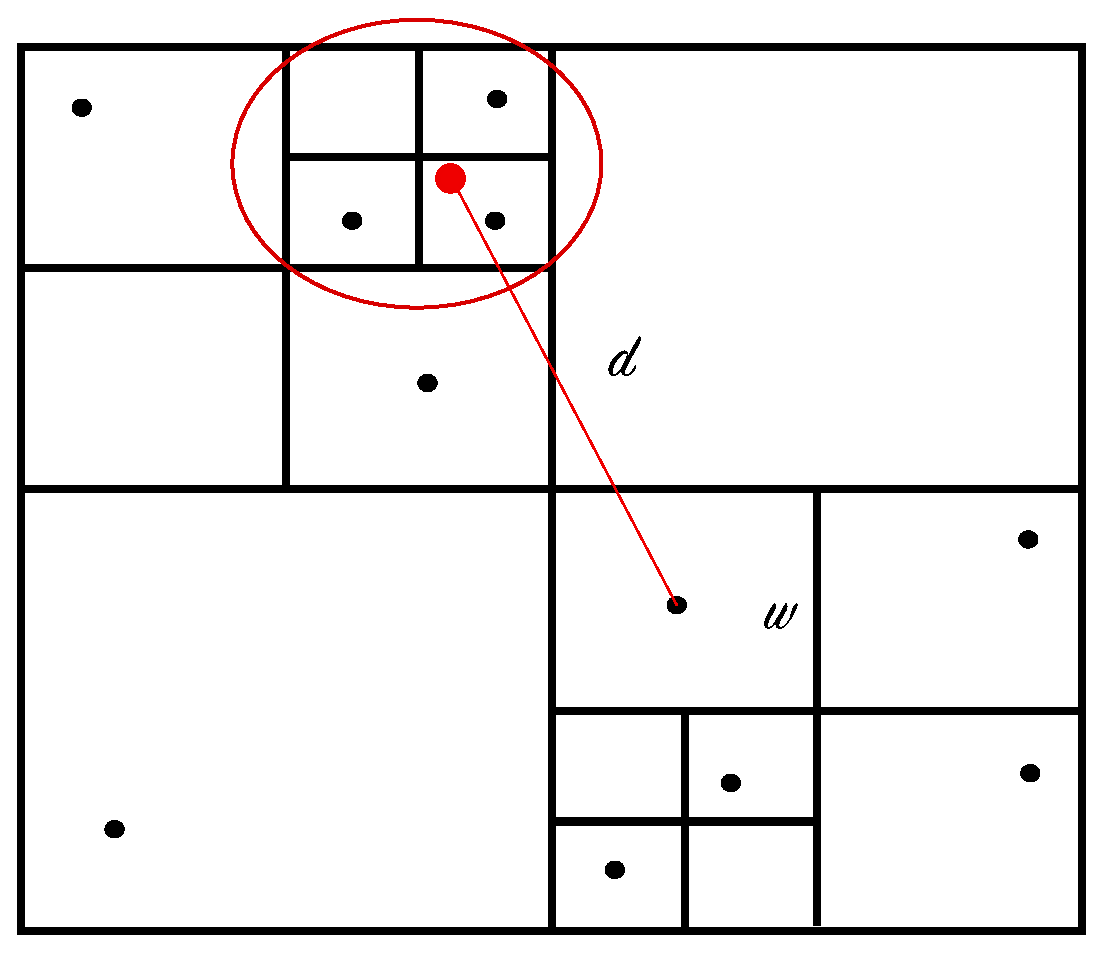
\includegraphics[scale=0.2]{figs/domain2.eps}}
  \hspace{1pt} 
  \subfloat[]{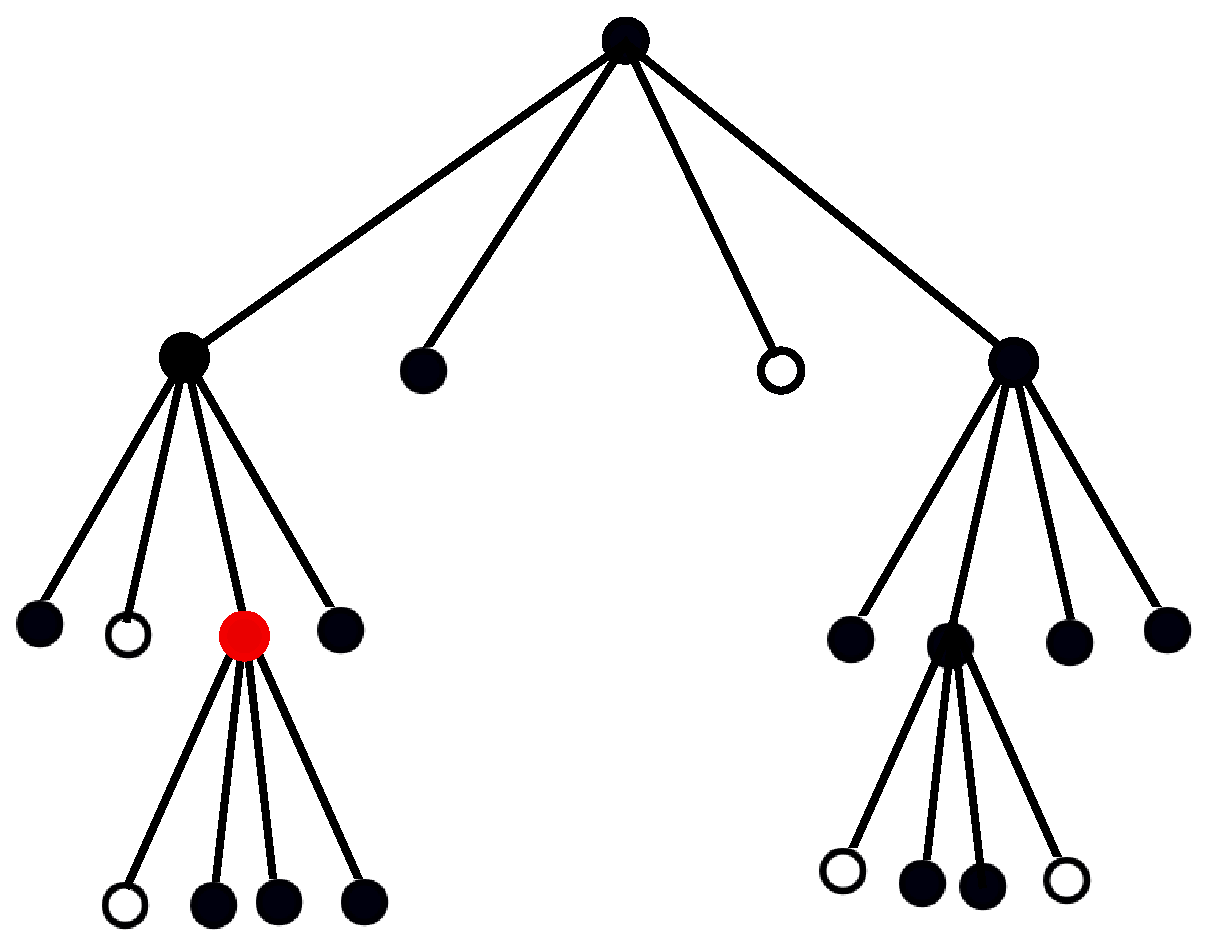
\includegraphics[scale=0.2]{figs/tree.eps}}
  \caption{(a) Set of bodies in  domain space. The red dot represents the particle (non-leaf node) that has the center of mass and total mass of the three circled particles (leaf nodes). (b) Corresponding Barnes-Hut quadtree.\label{domain}}
\end{figure}

\section{A Baseline Naive Implementation}\label{sec:yourmethod}
In this section we describe a parallel MPI \cite{mpi} implementation of the naive algorithm that we use as our baseline.

Implementing the naive algorithm allowed for a smooth introduction to the $N$-body problem. At the same time we have a baseline to ensure our Barnes-Hut implementation is efficient enough and exhibits the expected reduction in the asymptotic complexity of the problem.

Our approach consists of dividing the particles to equally sized disjoint subsets and letting each process compute the pairwise forces applied on them. The updated positions of the particles are distributed to every process at each step of the simulation using MPI collective communications.

Since the computation needed grows as $N^2$, we aimed for an implementation that is as performant as possible. Introducing Intel Intrinsics \cite{intel} for the computation intensive force calculation was one of our main optimizations. More specifically, we coded the entire force computation in AVX2.

\section{Parallelizing Barnes-Hut}\label{sec:barneshut}
In this section we describe the sequence of steps we took moving from a naive implementation to a parallel Barnes-Hut implementation.

\mypar{Division of Work} As already mentioned, the Barnes-Hut algorithm approximately computes the force on each particle starting from the root node of the tree and descending to every subtree. A multi-core implementation has to choose between two work division schemes, a particle-based one or a tree-based one. In the first scheme, each core is assigned a subset of the particles and computes the applied forces by taking into account the entire tree. In the latter, each core is assigned only a part of the whole tree and computes a part of the total force on every particle. \newline
\indent As a first step, we considered and implemented a simple tree-based work division scheme. Our approach consisted of creating the tree in the root process and then distributing its second level subtrees to the cores. However, an octree is unbalanced and has at most 64 second level subtrees, meaning that load balancing issues could arise. One possible solution would be to distribute the subtrees dynamically based on the load they impose. Of course this would not be enough in case of a very unbalanced tree, e.g., one subtree imposes as much work as the other 63. The distribution of the tree in such a way would also be problematic in the case of scaling to more than 64 cores. These problems could be alleviated by dividing the tree in a more sophisticated and dynamic way by taking into account the work required for each separate node. Considering the complexity of such a solution and the time limitations of the project we opted to experiment with particle-based schemes. \newline
\indent Opting for particle-based schemes however, does not automatically solve the challenge of load balancing, which stems from the central and most time consuming component of our problem, the force computation. We considered three alternative approaches to load balancing by dividing the domain in subdomains of equal area, equal number of particles and equal amount of work.

\mypar{Subdomains of Equal Area} Our first approach is splitting the domain in subdomains of equal area. Then each core has to compute the force applied on the particles of one such subdomain. \newline
\indent In a uniformly distributed particles setting, this approach generally results in good load balancing, since every processor is assigned more or less the same number of particles. However, this is hardly the case in the majority of real world simulations where the distribution of particles in the domain space is random. As a result, subdomains can have significantly different numbers of particles which most of the time translates to subpar load balancing.

\mypar{Subdomains of Equal Number of Particles} Naturally, our next step is to consider subdomains of equal number of particles. Instead of splitting the domain space in areas of equal size, we shift the split point to ensure that the subdomains include equal number of particles. \newline
\indent Such an approach guarantees that there will be no core with significantly less load than the others, but the load could still differ quite a bit. The cause is that two particles may require a different number of computations to approximate their net force, which depends on their distance from the others and on the parameter $\theta$. For the degenerate case of $\theta = 0$, great load balancing is achieved as the algorithm turns to brute force and no internal node is considered as a single particle.

\mypar{Subdomains of Equal Amount of Work} Identifying that the different amount of work required for different particles can lead to load imbalances, we now know our next move. This time we have to set the split point of the domain while having in mind that the produced subdomains should contain particles whose required work sums up to equal amounts. The work required for each particle is defined as the number of tree nodes traversed to compute its net force and is calculated in every step of the simulation. \newline
\indent Distributing the particles among cores in such a way should diminish load balancing inequalities. Each core will have equal or nearly equal amount of work to do and we expect this to hold, even for very large numbers of cores. 

\mypar{Implementation} We implemented our codes in C++, leveraging the power of MPI to parallelize them. As the Barnes-Hut algorithm requires irregular, dynamic communication patterns, one sided operations are used to avoid remote process synchronization. Every process exposes its local tree for other processes to directly read it using MPI\_Get operations. As each process recomputes its part of the tree in every simulation step, a dynamic memory window is used to avoid continuous allocation of memory windows. To support MPI operations on parts of the tree we serialize the tree data structure.

\mypar{Correctness} We validated the correctness of our implementations by using the law of conservation of energy, which requires that the total energy of the system is constant over the whole simulation. At the same time we compared our simulation results with NEMO \cite{nemo} for a set of fixed inputs. More precisely, we required that $\max_{i,t} \{\text{RE}_i^t\}$ should be smaller than a given threshold of $0.01 \%$, where $\text{RE}_i^t$ is defined as the relative error $|x_i^t - x_i^{t,\text{NEMO}}|/ |x_i^{t,\text{NEMO}}| $ in position coordinate $x$ of any particle $i$ at time $t$, and the same for the coordinates $y$ and $z$. We allowed a threshold to account for implementation differences, as our codes were not developed based on NEMO.

\section{Experimental Results}\label{sec:exp}
In this section we present experimental results for our baseline and more sophisticated Barnes-Hut implementations. The scalability of our best approaches is studied using strong and weak scaling benchmarks.
Finally, we compare to a well established optimized implementation and present a qualitative Roofline model benchmark of our most performant codes.

\mypar{Experimental Setup and Approaches} We ran all our experiments on the Euler cluster \cite{cluster} requesting up to 48 CPU cores and 1 gigabyte of RAM per core. More precisely, we used two Euler II compute nodes each equipped with two 12-core Intel Xeon E5-2680v3 processors (2.5-3.3 GHz) and DDR4 memory at 2133 MHz. We used the compiler GCC 6.3.0, with its -O3 option enabled and opted for MVAPICH 2.2, as it was the only available MPI implementation that fully supported the RMA operations we needed. 

For our experiments we use a time-step of $0.0001$ and $\theta = 0.5$. Initially the particles are randomly distributed in a unit sphere. Starting from a cold cache we measure the time taken to execute 5 time-steps.

Time measurements were done using the MPI\_Wtime command and MPI\_Barrier was used to synchronize processes in order to time specific program sections. The median of the measurements was chosen as more representative over the maximum. As the Q-Q plot deviated strongly from the expected linear relation, the hypothesis that the measurements adhere to a normal distribution was rejected. We computed 99\% confidence intervals of the median and not the mean. However, they were very narrow, implying that our measurements were nearly deterministic. Moreover, an experiment that ran $n$ times on $p$ processors resulted in $n*p$ measurements of which only one was kept for our analysis as the Kruskal-Wallis test with $\alpha=0.05$ rejected the hypothesis that these values belong to the same population.

\mypar{Overview} We begin with a comparison of our two best approaches, Barnes-Hut with load balancing based on equal number of particles and on equal amount of work, and our optimized naive baseline with vector instructions. The total execution time of all the approaches for a problem size of $130k$ is presented In Fig.~\ref{overview}. Our Barnes-Hut codes prove to be at least one order of magnitude faster than our fastest baseline. Going to larger problem sizes we expect that the baseline code would not be able to keep up. However, the Barnes-Hut codes do not scale as well as our baseline as we increase the number of cores. The reasons behind this are further examined in the rest of our report.

\begin{figure}[h]
 \centering
  \caption{Total execution time of our baseline and best approaches.\label{overview}}
  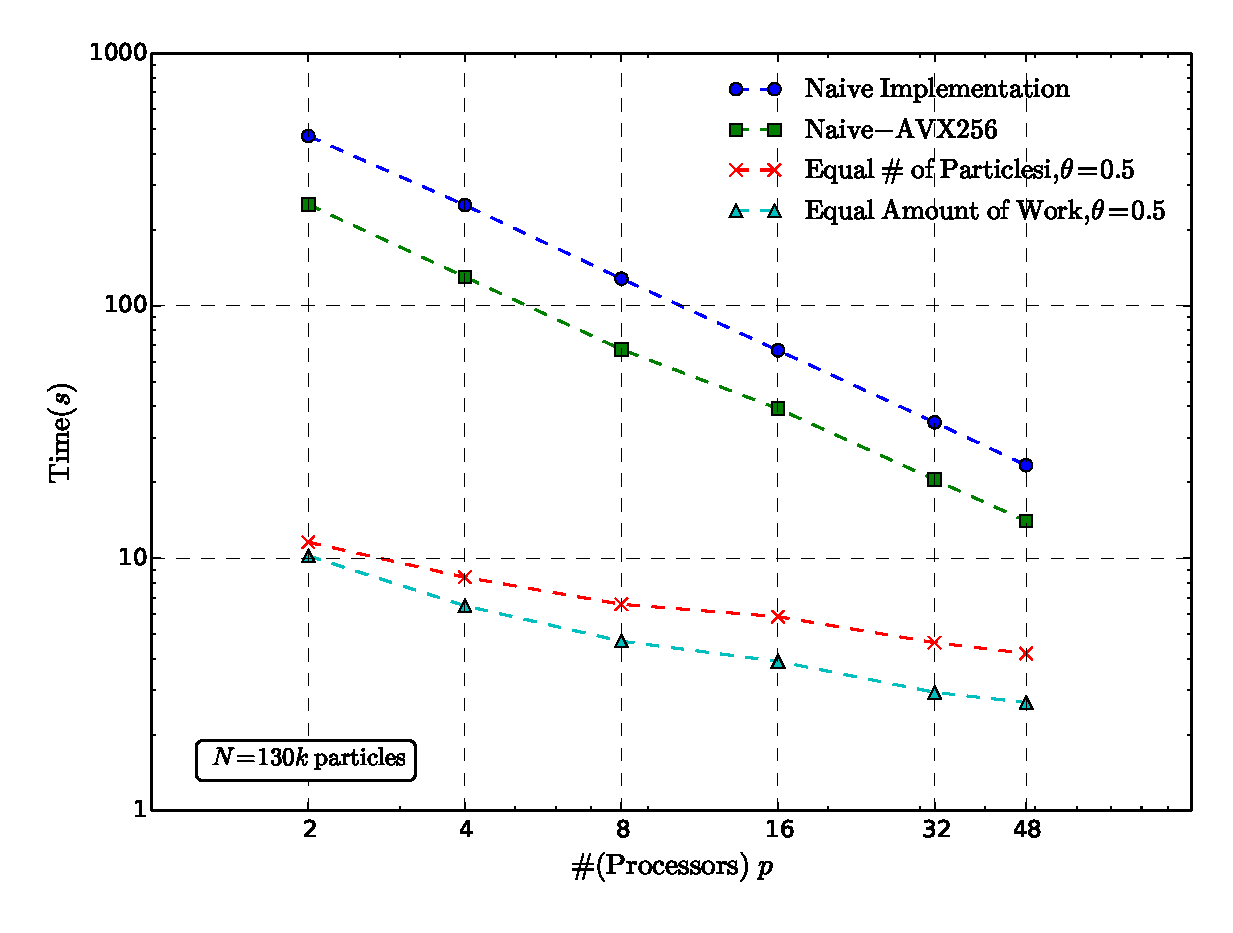
\includegraphics[scale=0.4]{figs/130kComparison.eps}
\end{figure}

\mypar{Baseline Performance}
Investigating the performance and scalability of our baseline, we compared its run time to the theoretical best and to that of our baseline code without vector instructions. The total execution time for a problem size of $130k$ is shown in Fig.~\ref{totalAVX}.

\begin{figure}[h]
 \centering
  \includegraphics[scale=0.4]{figs/total.eps}
  \caption{Experimental and theoretical running times of our non-vectorized and vectorized baselines.\label{totalAVX}}
\end{figure}

Both versions follow the same trend in which the execution time is nearly halved as the number of cores is doubled. For a fixed number of cores, the vectorized version is faster by $1.8$ times on average. This improvement differs greatly from the best theoretical speedup of $4$ times that AVX2 can offer. Running on an Euler V compute node (Intel Xeon Gold 5118) we observed an improvement of $3$ times proving that the CPU was the main limiting factor. The theoretical best was not reached most likely due to the unavoidable use of high latency instructions such as division.

To further examine the performance of our baseline we compare the experimental execution time with the theoretical one obtained from \textit{Amdahl's Law} with $f {=} 0$. As shown in Fig.~\ref{totalAVX} the two are very close, but the gap between them widens as we increase the number of cores due to added communication overhead, which is not accounted by \textit{Amdahl's Law}.

\mypar{Barnes-Hut Strong Scaling}
Fixing the problem size to $N{=}524k$, we compare our two best Barnes-Hut codes. In Fig.~\ref{Comparison}, we present the speedup for the equal number of particles and equal amount of work load balancing approaches with the base case being one parallel process.

\begin{figure}[h]
 \centering
  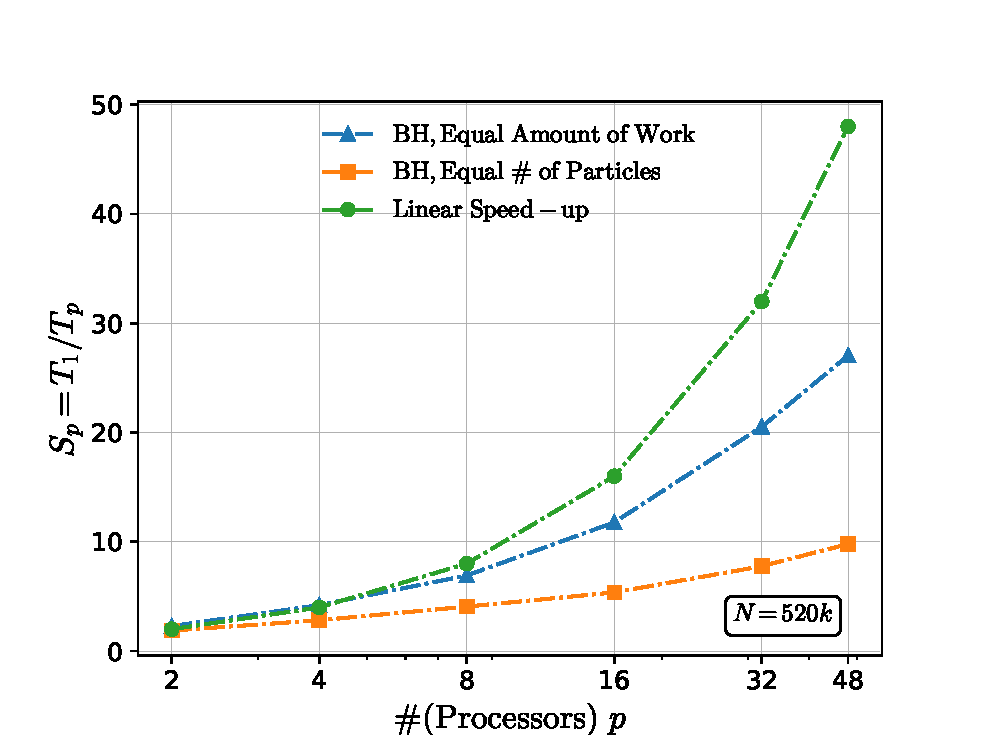
\includegraphics[scale=0.4]{figs/SpeedupNew.eps}
  \caption{Speedup of our equal number of particles and equal amount of work Barnes-Hut implementations.\label{Comparison}}
\end{figure}

The equal amount of work optimization rewards us with a much better parallel speedup than the subpar equal number of particles approach. The speedup exhibited by this code on up to 8 cores is very close to linear. However, this approach too falls short of our expectations as we successively increase the number of cores.

\begin{table}[h]
\scriptsize
\begin{tabular}{|l|c|c|c|c|c|c|c|}
\hline
\# Cores          & 1       & 2      & 4      & 8     & 16    & 32    & 48    \\ \hline
Exec.         & 653.20  & 286.38 & 155.38 & 94.44 & 55.46 & 31.82 & 23.15 \\ \hline
Comp.      & 647.41  & 281.66 & 149.19 & 83.83 & 42.29 & 20.28 & 13.48 \\ \hline
Comm.    & 7.6e-05 & 1.09   & 2.37   & 4.43  & 7.75  & 7.10  & 6.81  \\ \hline
Tree & 5.29    & 2.17   & 1.12   & 0.68  & 0.33  & 0.14  & 0.12  \\ \hline
\end{tabular}
\caption{Total execution, computation, communication and tree construction time (seconds) of the equal amount of work code.}
\vspace{-5pt}
\label{tab::strong}
\end{table}

As shown in Table 1, the computation and tree construction time halve as we double the number of processors. In contrast, the communication time doubles as we double the number of cores until we reach 16, explaining why the observed speedup is not ideal.

\mypar{Barnes-Hut Weak Scaling}
We further investigate the scalability of our best implementation by performing a weak scaling benchmark in which we fix the number of particles per core to $65k$, amounting to $3m$ particles on 48 cores. As shown in Fig.~\ref{weaksc}, the communication overhead increases linearly as we increase the problem size. On 48 cores, the communication time constitutes nearly one third of the total execution time, making it a first class target for future optimization. On the other hand, the tree construction time remains stable and the computation time increases slowly as expected due to the approximate complexity of $NlogN$ induced on the problem by the Barnes-Hut algorithm.

\begin{figure}[h]
 \centering
 \includegraphics[scale=0.4]{figs/weak.eps}
  \caption{Time for different parts of the code (equal amount of work) in a weak scaling benchmark.\label{weaksc}}
\end{figure}

%%To eliminate this, the next step would be to serialize the tree structure used in our algorithm. This would allow us to share the %%tree more efficiently between processors. Specifically the tree wouldn't have to be broadcast in its entirety to each processor in %%every step but each processor could request only a certain number of nodes that it needs to perform the next computation, leaving
%% away the more precise information about mass and location of far away particles found further down in the tree.

\mypar{Roofline Benchmark}
To further examine the performance of our codes, we resorted to a roofline benchmark. To be able to do at least a qualitative benchmark we had to use a different machine (Intel Core i7-2820QM, 2.30GHz x 8 CPU), as Euler cluster CPUs do not provide FLOPS hardware counters. For the measurements of LLC cache misses and number of cycles one compute node of our original setup was used. We assumed that the FLOPS counted on the new machine are comparable to the ones we would measure on the Euler cluster. Memory bandwidth was set to 68 GB/s according to Intel's product sheet but was not multiplied by 8 when considering 8 cores, since the LLC is shared. In contrast, the estimated peak performance of 2.5GHz x 16 FLOPS per cycle was multiplied by 8. Due to memory constraints our experiments were performed on particle sets of sizes 128, 256, 512, 1024, 2048, 4096, 8192, 16384, 32768 and 65536. The results are presented in Fig.~\ref{roofline}.

\begin{figure}[h]
 \centering
 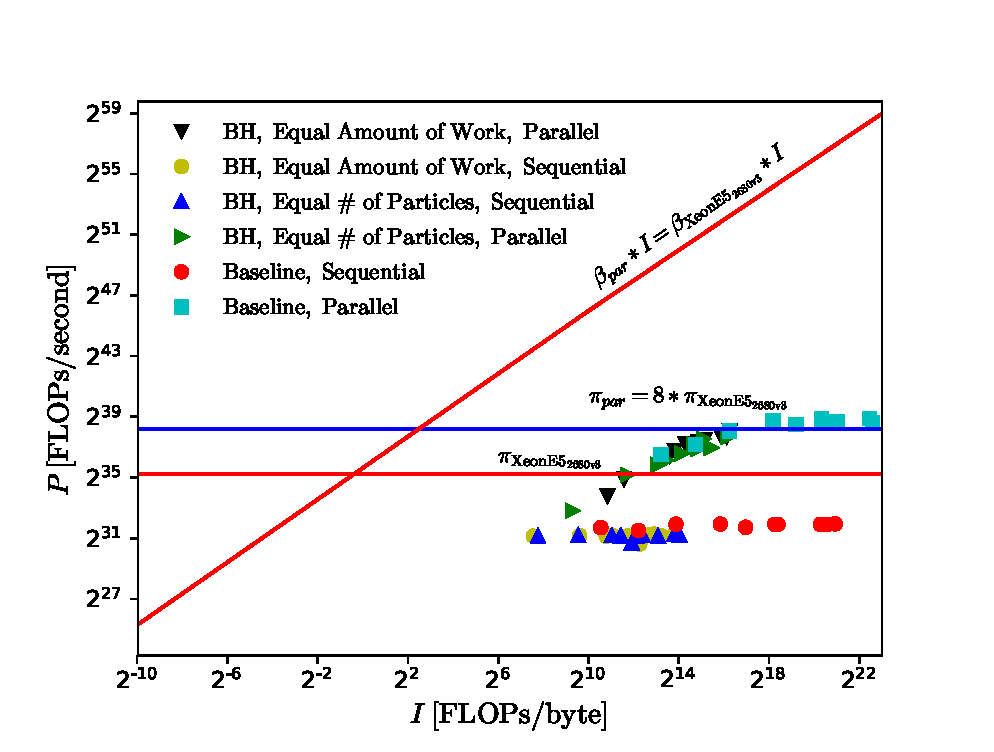
\includegraphics[scale=0.4]{figs/roofline.eps}
  \caption{Qualitative Roofline model plot on 1 and 8 cores.\label{roofline}}
\end{figure}

Our best two Barnes-Hut approaches exhibit lower operational intensity compared to our baseline. Such a result is expected as the Barnes-Hut algorithm operates on a tree data structure, which inevitably increases the number of bytes read per FLOP executed. However, lower intensity is welcomed when it is accompanied by lower running time due to the Barnes-Hut approximation, whose aim is to reduce the total work done, i.e., the executed FLOPS. 

The fact that the parallel baseline exceeds peak performance could be due to the baseline CPU frequency being lower than the actual one. Nevertheless, it could also be that the hardware counters over-count FLOPS in the parallel setting. This means our parallel implementations could prove to be memory bound for smaller particle sets, which however is not alarming as we are interested in larger sets.

Regarding the gap between the experimental performance and the theoretical peak performance in the sequential setting, we have to mention that our codes include division operations, which count as one FLOP but could take multiple cycles, thus keeping the FLOPS/cycle down.

\mypar{Real World Benchmark}
To examine if our approach matches the trends of real world implementations, we chose to compare it to the cosmological simulation code Gadget 2 \cite{gadget}. Gadget 2 is able to simulate $N$-body systems using a multipole expansion tree algorithm that is comparable to the Barnes-Hut algorithm due to its inherent tree structure. Since Gadget 2 is used for different types of simulations we ran it without any special types of particles and without periodic boundary conditions. Gadget 2 was compiled and run using GCC 4.8.2 and OpenMPI 1.6 as recommended. In Fig. \ref{gadget}, we present a weak scaling benchmark of Gadget 2 and our most successful implementation, Barnes-Hut with load balancing based on needed work. We successively increased the number of cores and particles proportionally, starting from $65k$ particles for one core.

\begin{figure}[h]
 \centering
 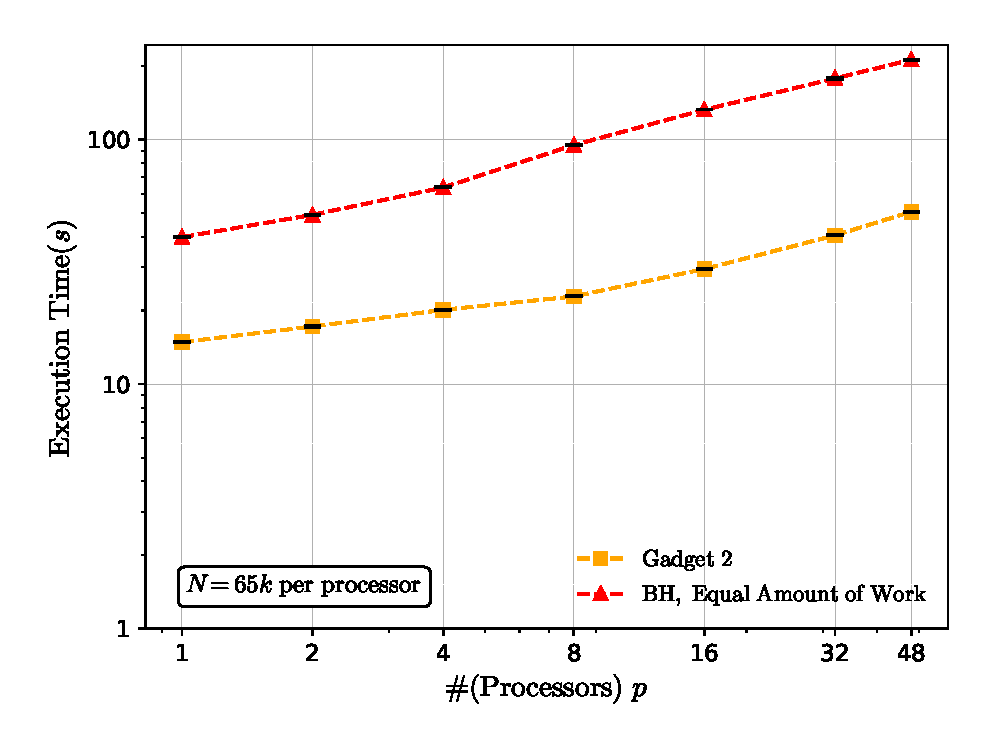
\includegraphics[scale=0.4]{figs/gadget_benchmark.eps}
  \caption{Runs for our own code compared to Gadget 2 in a weak scaling benchmark.\label{gadget}}
\end{figure}

The general trends of the two implementations coincide, showing a growing parallelization overhead. However, our code proves to be 2 to 3 times slower mainly due to the multipole expansion tree algorithm reducing the complexity of the problem to $N$. This explains why the gap in execution time widens as we go over to more processors and more particles. The growing difference in execution time could also be partially attributed to the communication overhead imposed by our implementation of the Barnes-Hut algorithm, as seen in Fig.~\ref{weaksc}.

\section{Future Work}

In this section we discuss possible improvements to our implementations based on our observations and experimental measurements.

As presented in Section 5, our codes suffer from a growing communication overhead when the number of cores is increased. One possible optimization would be to dynamically request only the needed parts of the tree owned by other processes when computing the net force on a particle. Of course, this would require a way of caching parts of the tree to avoid needless communication when two particles require the same parts. Another improvement would be to overlap communication with computation by keeping a queue of needed tree parts, which are prefetched using asynchronous communication operations while the main computation occurs.

\section{Conclusions}

Even though the $N$-Body problem has been around for a long time, researchers still attack it with new ideas and optimizations. In our approach we attempted to efficiently parallelize the Barnes-Hut algorithm in a multi-core distributed memory setting. We experimented with MPI RMA and implemented different load balancing techniques. We explained why load balancing based on equal amount of area and equal amount of particles might fall short and how balancing based on equal amount of work solves their deficiencies. Our Barnes-Hut implementations strongly outperformed our optimized naive baseline that also used Intel Intrinsics. Finally, despite the deficiencies we identified in our best approach, the comparison to the more sophisticated Gadget 2 code proved that our code performs well with respect to the complexity that the two codes induce on the $N$-Body problem.

% References should be produced using the bibtex program from suitable
% BiBTeX files (here: bibl_conf). The IEEEbib.bst bibliography
% style file from IEEE produces unsorted bibliography list.
% -------------------------------------------------------------------------
\bibliographystyle{IEEEbib}
\bibliography{bibl_conf}

\section{Appendix}

\mypar{Source Code Repository}
All of our code and benchmark results can be found in the following Github repository:
\textit{https://github.com/ktrianta/n-body-problem/}

\end{document}

